\documentclass{beamer}

% Setup appearance:

\usetheme{Darmstadt}
\usefonttheme[onlylarge]{structurebold}
\setbeamerfont*{frametitle}{size=\normalsize,series=\bfseries}
\setbeamertemplate{navigation symbols}{}


% Standard packages

\usepackage[brazil]{babel}
\usepackage[latin1]{inputenc}
\usepackage{times}
\usepackage[T1]{fontenc}
\usepackage[table]{xcolor}
 
% Setup TikZ

\usepackage{tikz}
\usetikzlibrary{arrows}
\tikzstyle{block}=[draw opacity=0.7,line width=1.4cm]

%diretório das figuras
\graphicspath{../article}

\title[Tegra 3]{%
Processador NVidia Tegra 3%
}

\author[Souza,Santos,Ara\'ujo]{
     Danilo~Souza\and
     Hugo~Santos\and
     Welton~Ara\'ujo
     }


\institute[Bel\'em]{
  \inst{1}%
  Universidade Federal do Par\'a
  }
\date[Bel\ém 2012]{
  29 de Junho de 2012
  }



\begin{document}

\begin{frame}
  \titlepage
\end{frame}

\begin{frame}{Agenda}
  \tableofcontents
\end{frame}

\section{Introdu\c{c}\~ao}
\begin{frame}{Introdu\c{c}\~ao}
  \begin{itemize}
    \item	PIC 16F628A
    \item	Simular o jogo do choque
  \end{itemize}
    \begin{figure}[ht]
      %\centering
      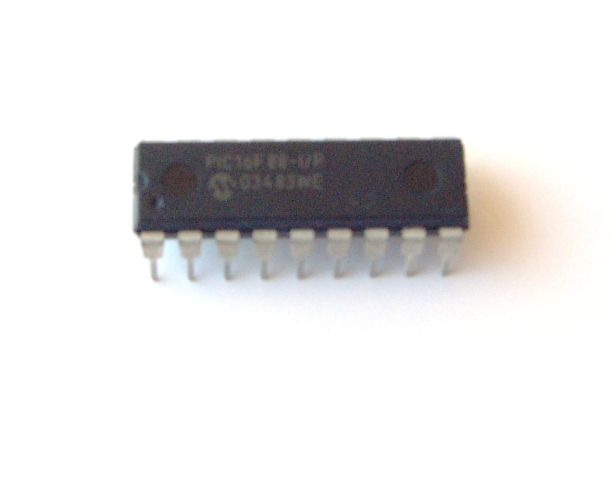
\includegraphics[width=5.0cm]{./article/pic18dil.jpg} \quad
      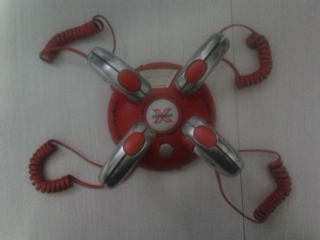
\includegraphics[width=5.0cm]{./article/dispositivo1.png}
  \end{figure}
\end{frame}

\section{Descri\c{c}\~ao do Jogo}
  \begin{frame}{Descri\c{c}\~ao do Jogo}
	\begin{itemize}
	  \item 	2 a 4 jogadores
	  \item		1 controle por jogador
	  \item		LED vermelho piscando indica o come\c{c}o da rodada
	  \item		LED verde aceso indica o fim da rodada
	  \item		O \'ultimo jogador a apertar o bot\~ao leva choque
	\end{itemize}
	\begin{figure}[ht]
	  \centering
	  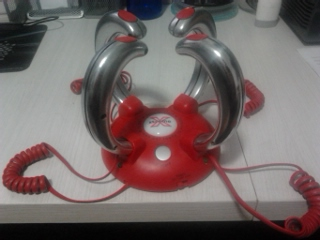
\includegraphics[width=7.0cm]{./article/dispositivo2.png}
	\end{figure}
  \end{frame}
   
\section{Descri\c{c}\~ao da Simula\c{c}\~ao}
  \begin{frame}{Descri\c{c}\~ao da Simula\c{c}\~ao}
	\begin{itemize}
	  \item 	2 a 4 jogadores
	  \item		1 bot\~ao por jogador
	  \item		2 LED's por jogador
	  \item		LED vermelho aceso indica o começo da rodada
	  \item		LED vermelho apagado o fim da rodada
	  \item		O \'ultimo jogador a apertar o botão leva choque
	  \item		LED amarelo indica que o jogador levou um choque
	  \end{itemize}
  \end{frame}

  \subsection{O algoritmo}
    \begin{frame}
      \begin{itemize}
	\item	Escolher n\'umero de jogadores
	\item	Pressionar \textit{START}
	\item	Esperar LED vermelho apagar
	  \begin{itemize}
	   \item	Caso um bot\~ao seja pressionado antes, este levará um choque
	  \end{itemize}
	\item	Checar se algum bot\~ao foi pressionado
	  \begin{itemize}
	    \item	Incrementar contador caso algum bot\~ao tenha sido pressionado
	  \end{itemize}
	\item	Checar quais bot\~oes foram pressionados
	\item 	Dar choque no pino do \'ultimo bot\~ao pressionado
      \end{itemize}
    \end{frame}
    \begin{frame}
      \begin{figure}[ht]
	  \centering
	  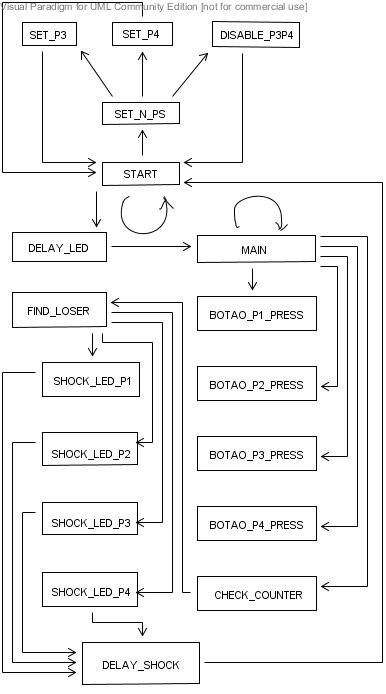
\includegraphics[width=7.0cm]{./article/fluxograma.jpg}
      \end{figure}      
    \end{frame}

\subsection{A Simula\c{c}\~ao}
    \begin{frame}
     \begin{figure}[ht]
	  \centering
	  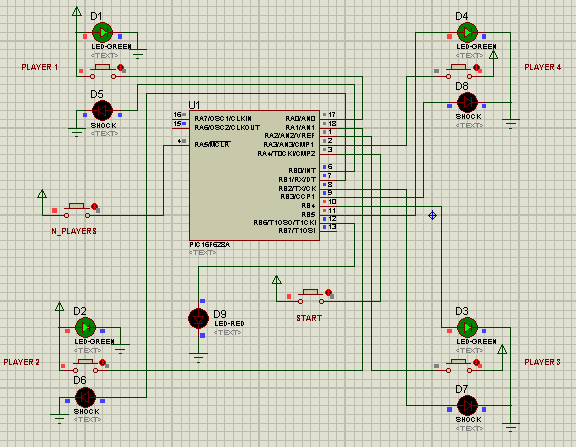
\includegraphics[width=7.0cm]{./article/4jogadores.png}
      \end{figure}
    \end{frame}
    \begin{frame}
     \begin{figure}[ht]
	  \centering
	  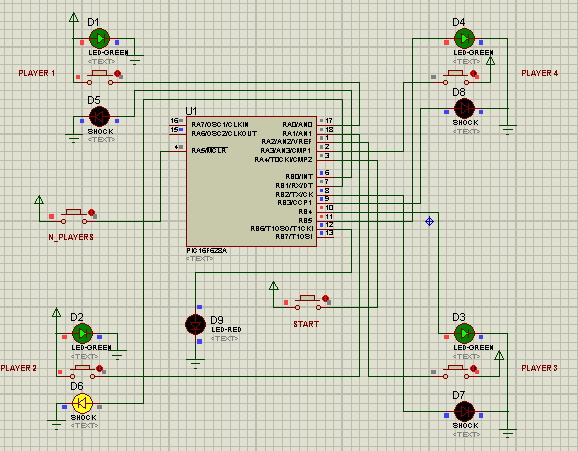
\includegraphics[width=7.0cm]{./article/choqueP2.png}
      \end{figure}
    \end{frame}
        \begin{frame}
     \begin{figure}[ht]
	  \centering
	  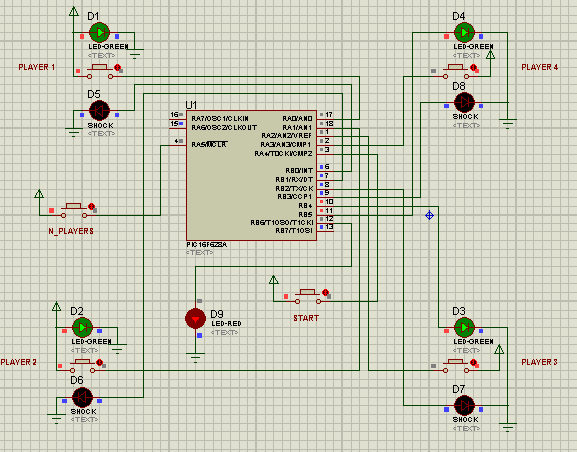
\includegraphics[width=7.0cm]{./article/delaystart.png}
      \end{figure}
    \end{frame}

  \end{frame}

  

\end{document}
